\documentclass[conference]{IEEEtran}
\usepackage{cite}
\usepackage{amsmath,amssymb,amsfonts}
\usepackage{graphicx}
\usepackage{textcomp}
\usepackage{xcolor}
\usepackage{booktabs}
\usepackage{multirow}
\usepackage{hyperref}

\usepackage{url}

% Unnumbered footnote for the artifact pointer on page 1.
\newcommand\blfootnote[1]{%
  \begingroup
  \renewcommand\thefootnote{}\footnote{#1}%
  \addtocounter{footnote}{-1}%
  \endgroup
}

\begin{document}
% Long model paths and URLs in a narrow IEEE column overflow under default tolerances;
% prefer loose interword spacing over text in the gutter.
\sloppy

\title{Following the Speedup: An Audit of Adaptive\\ Draft Length in Speculative Decoding}

\author{
% Titles dropped: ML venues do not use them in the byline. Affiliation line removed at the
% authors' request, and the \IEEEauthorrefmark superscripts went with it since there is no
% longer a block for them to point at. Without honorifics the six names fit one line.
\IEEEauthorblockN{Pramod Kumar Reddy Jella,
Yash Dixit,
Naman Dwivedi,
Raj Dandekar,
Rajat Dandekar,
Sreedath Panat}
}

\maketitle
\blfootnote{Code, raw per-run JSON, and the benchmarking protocol:
\url{https://github.com/pramodjella/speculative-decoding-draft-length-audit}}

\begin{abstract}
Adaptive draft length promises a double-digit speedup, and the published strategies do not
deliver it. We establish a tuned fixed-length baseline, then a Bayes ceiling on what any
draft-side signal could add on top of it, and most of the promised gain turns out to sit above
that ceiling: unreachable, not merely unreached. The practical consequence is blunt. Reported
adaptive gains fall below the ceiling, and a tuned fixed draft length already reaches that
far, so the effort spent on signal-based adaptive length buys little that tuning does not.
We show this by following the promised gain through three gates. Published oracle arguments
put the prize at $+12$ to $23\%$ over any fixed draft length. Gate one asks whether the gain exists: a Bayes-ceiling decomposition
attributes about $80\%$ of it to verification-outcome variance that the draft-side state does
not determine, which leaves roughly $+3\%$ for any policy reading that state. Gate two asks what could reach the remainder. Cheap logit
features recover almost none of it and token position recovers exactly none, but the drafter's
hidden state does carry the signal, at AUC $0.79$ to $0.88$. Gate three puts that signal in a
running engine, where acting on it costs $2$ to $17\%$ against a tuned fixed depth. One policy
survives the audit: signal-free saturation tail-pruning, worth $+2$ to $5\%$ at batch size~1,
with one of three workloads a wash and the gain gone by batch~8. Seeing the leak at all
required fixing six evaluation practices that inflate adaptive-length results, including
unpaired GPU timing that gave us three contradictory answers from identical configurations.
We release the protocol, the code, and the raw per-run measurements.
\end{abstract}

\begin{IEEEkeywords}
speculative decoding, adaptive draft length, per-step acceptance signal, hidden-state probe, oracle decomposition, benchmarking methodology, EAGLE, efficient inference, LLM serving.
\end{IEEEkeywords}

\section{Introduction}
Speculative decoding (SD) speeds up generation by having a cheap draft model propose $K$
tokens that the target then verifies in a single parallel pass \cite{leviathan2023spec,chen2023spec}.
The draft length $K$ is the primary tuning knob. Too short a draft leaves speedup unclaimed;
too long a draft spends compute on tokens the target will reject. A large literature therefore
proposes setting $K$ per step from some decode-time signal.

The case for doing so rests on an oracle argument. Suppose the number of tokens the target
will accept were known in advance, and the drafter proposed exactly that many. Throughput
would rise by double digits over any fixed $K$. SpecDecode-Bench \cite{specdecodebench} recently made this concrete
on vLLM, establishing that verification dominates SD execution, that accepted length swings
widely across positions and requests, and that a wide gap separates deployed methods from the
oracle. It closed with a call for ``a lightweight predictor that can adaptively
select\ldots approaching the oracle bound.''

We began by trying to build a better draft-length policy, following where the research was
heading. What stopped us was more basic. We could not reproduce the speedups the papers
reported. In our own harness, Python-side overhead was large enough to swamp the effect we
were trying to measure. The numbers we could produce matched neither the published ones nor
what vLLM already delivers. So the question changed. Before asking which policy wins, we
had to work out how to measure speedup honestly, how much is genuinely available, and why the
field is moving in the direction it is. This paper is that measurement, and
Fig.~\ref{fig:waterfall} is its whole argument in one picture: the promised gain, and what
each stage of the audit removes from it.

The oracle number is the speedup available to a drafter that knows exactly how many of its
proposed tokens the target will accept. That is knowledge of the future, not a policy, and the
distinction carries most of what follows.

% Column width, not figure*: a full-width float can only sit at the top of a page, and page
% one's top belongs to the title block, so figure* pushes this to page two. It is the opening
% picture of the argument and needs to be on page one. The PNG is drawn at a matching aspect
% ratio so it stays legible at this size.
\begin{figure}[t]
\centering
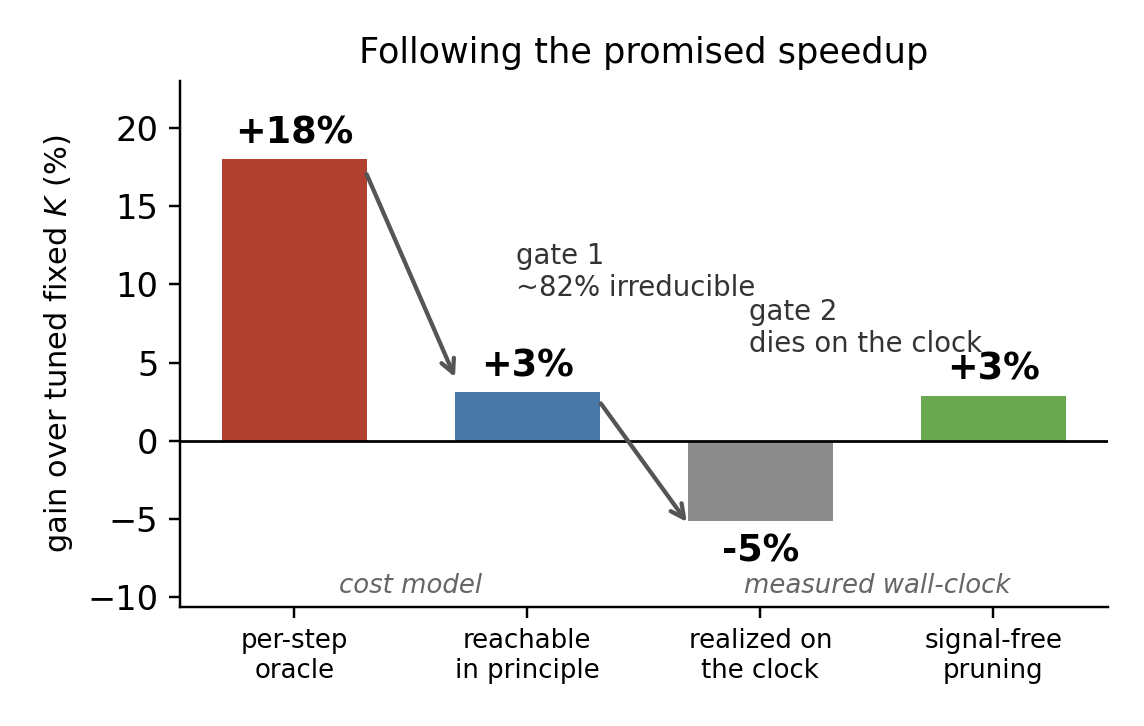
\includegraphics[width=\columnwidth]{figures/fig_waterfall.png}
\caption{The audit in one picture. The oracle promises $+18\%$ on this model. Most of it is
irreducible from any draft-side signal, and what remains inverts sign once a real engine has
to execute the policy. The survivor at right reaches a similar height by a different route,
using no learned signal at all. The first two bars are cost-model figures on the Llama-3.1-8B
ladder and the last two are measured wall-clock, which is the point: the promise is scored in
one currency and the delivery in another.}
\label{fig:waterfall}
\end{figure}

\subsection{The audit}
We follow the claimed number through three gates, each of which removes part of it
(Fig.~\ref{fig:waterfall}).

\emph{Gate 1, is the gain there at all?} We decompose the per-step oracle into what a tuned
fixed $K$ already collects, what a draft-side signal could still reach, and what is
irreducible. About $80\%$ falls in the last bucket. The oracle overstates the achievable prize
by roughly five times (\S\ref{sec:gate1}).

\emph{Gate 2, can any real signal reach the rest?} The reachable slice is genuinely there, and
we find where it lives. It is not in the cheap logit features the literature has used, which
recover $+0.3$ to $8\%$ of the span, nor in token position, which recovers exactly zero. It is
in the drafter's hidden state, from which a PCA and logistic probe recovers about a fifth of
the oracle span (\S\ref{sec:gate2}). This closes a door rather than opening one. We looked in
the best remaining place and the answer was still no.

\emph{Gate 3, does it survive execution?} We put the signal in a live engine. Every learned or
entropy-based stopping policy we tested loses to a tuned fixed depth, by $2$ to $17\%$
(\S\ref{sec:gate3}). The offline arithmetic and the wall clock disagree because drafting is
cheap and verification is not, so stopping early saves little and forfeits a lot.

What survives is one policy that uses no signal: stop drafting when the cumulative path
probability saturates. It is worth $+2$ to $5\%$ at batch size 1, and the mechanism explains
why it works where prediction fails (\S\ref{sec:survivor}).

\subsection{Why this was not visible earlier}
The effects in this area are a few percent, and at that scale the measurement apparatus
decides the answer. Six practices, each common and each individually reasonable, inflate
adaptive-length results. We encountered all six. The worst was unpaired sequential timing, which
returned $+2.4\%$, $-1.9\%$ and $+6.4\%$ from identical configurations before we started
pairing. Table~\ref{tab:failuremodes} lists them with what each one did to our own numbers.
The protocol we ended up with is the instrument that made the rest of the audit readable, so
we describe it before the results (\S\ref{sec:protocol}) rather than as a separate finding.

Every comparison here concerns speed at unchanged output, since exact-verification SD is
lossless.

\section{Related Work}
\emph{Feature-based drafting.} EAGLE-1/2/3 \cite{li2024eagle,li2024eagle2,li2025eagle3} draft
from the target's hidden states. EAGLE-2 and 3 adapt the tree shape using draft confidence but
still commit to a static depth. TALON \cite{talon} fits tree structure to a token budget.

\emph{Signal-based length control.} SVIP \cite{zhang2024svip}, AdaEDL \cite{adaedl} and DSDE
\cite{dsde} stop drafting on entropy, margin or KL thresholds.

\emph{Learned controllers.} SpecDec++ \cite{specdec} trains an acceptance head and DISCO
\cite{disco} a classifier. BanditSpec \cite{hou2025banditspec} and its successors treat $K$ as
a bandit arm.

\emph{Cumulative-confidence stopping.} SADDLE \cite{saddle}, PACER \cite{pacer} and DDD
\cite{ddd} stop on accumulated acceptance probability. This is the class our audit leaves
standing.

\emph{Serving-level adaptation.} Nightjar \cite{nightjar} and TurboSpec \cite{turbospec} gate
speculation by system load. That is a different lever, and a profitable one.

\emph{Benchmarking.} SpecDecode-Bench \cite{specdecodebench} established verification
dominance, the oracle gap and acceptance variance on vLLM. We credit those findings and claim
only our delta: splitting that gap into reducible and irreducible parts, locating the
reducible part, testing it on a clock, and the protocol that made the test trustworthy.

\emph{Baselines.} Most adaptive-$K$ papers compare against $K{=}1$ or an untuned default.
Measured against a per-workload tuned fixed $K$, their reported $2$ to $8\%$ gains fall inside
the $+2\%$ per-request oracle we measure (\S\ref{sec:supporting}).

\section{Setup}
\label{sec:setup}
\emph{Models.} Llama-3.1-8B-Instruct with \texttt{yuhuili/\allowbreak EAGLE3-LLaMA3.1-Instruct-8B};
Qwen3-14B with \texttt{AngelSlim/\allowbreak Qwen3-14B\_eagle3}; DeepSeek-R1-Distill-Llama-8B with
\texttt{yuhuili/\allowbreak EAGLE3-DeepSeek-R1-\allowbreak Distill-LLaMA-8B}.

\emph{Engine.} vLLM 0.23 (V1) on an H100, greedy, $B{=}1$ unless stated. Verification is
exact, so decoding is lossless; fp32 outputs are token-identical to the non-speculative
baseline. The wall-clock experiments use the SafeAILab/EAGLE-3 reference implementation
because vLLM exposes no per-step draft-length hook.

\emph{Workloads.} HumanEval, GSM8K and MT-Bench. Sample sizes differ by experiment and we
state them explicitly, since they are small. The hidden-state capture behind the decomposition
uses 30 prompts per workload at 128 max new tokens, which yields 41K to 60K labelled draft
positions per model. The wall-clock experiments use 10 prompts per workload for threshold
selection and probe training and a disjoint 10 for benching, also at 128 max new tokens, with
8 per workload in the batched runs. Repetition rather than prompt count carries the precision
in the timing results: 3 repeats in the policy zoo, 4 rotated cycles under the paired protocol,
and 3 fresh containers for the fair-baseline replication. Competition math
(MATH-500/AIME) serves as a reasoning control, and QuALITY 8K passages as a long-context one.

\emph{Baseline.} The best fixed $K$ by grid search over $K\in\{1..7\}$, tuned per workload.
On Llama-3.1-8B mixed traffic this lands at $K{=}2$ and $1.54\times$ measured net speedup.
This is a deliberately hard baseline, and most of what follows depends on it being hard.

There is a fair objection to it, which we should meet before the results rather than after.
Tuning $K$ per workload assumes the workload is known in advance, and a deployment serving
mixed traffic does not know that. On this reading our baseline gets something for free that an
adaptive method has to earn, and the comparison is unfair to adaptation. Our own data answers
this. The per-request oracle, which is exactly the gain available to a method that identifies
the right depth for each request without being told, is $+2.0\%$ over the globally tuned
$K$. Even perfect per-request adaptation therefore recovers about two percent, so a tuned
fixed depth is not merely a convenient baseline; it is close to the best that request-level
knowledge can buy. Where per-workload tuning is genuinely impossible, that $+2.0\%$ is the
prize on offer, and \S\ref{sec:supporting} shows online bandits failing to collect it.

\emph{Capture.} Hooks on the EAGLE3 draft head's \texttt{compute\_logits} record the full
per-position draft hidden state, 4096 or 5120 dimensions, 41K to 60K positions per model, with
per-step acceptance labels $\texttt{accept}[j] = [\texttt{acc} > j]$.

\emph{Two oracles.} We use two, and they differ by a lot, so we separate them here. The
\emph{per-step} oracle may change $K$ at every decode step, knowing exactly how many tokens
the target will accept at that step. It is worth $+12$ to $23\%$ over a tuned fixed $K$ and it
is the number the literature's motivating plots show. The \emph{per-request} oracle must
commit to a single $K$ for a whole request, but gets to pick the best one for that request. It
is worth only $+2.0\%$. The gap between the two is the value of reacting within a request,
and \S\ref{sec:gate1} is about how much of that value any real policy can capture.

\emph{Notation.} $K$ is the draft length in the chain regime, or tree depth. For a decode
step, $\mathrm{acc}\in\{0,\dots,K\}$ counts the drafted tokens the target accepts, so the step
emits $\mathrm{acc}{+}1$ tokens, and $\mathrm{MAT}$ is $\mathbb{E}[\mathrm{acc}{+}1]$. The
constant $C$ is the draft-to-target per-token cost ratio: one draft forward costs $C$ target
forwards, so a $K$-token step costs $1{+}CK$.

\emph{Cost model.} Offline policies are scored with $\mathrm{speedup} = \mathrm{MAT}/(1+CK)$.
We fit $C$ instead of assuming it. Setting $\mathrm{net}(K) = \mathrm{accept\_len}(K)/(1+CK)$
against the measured fixed-$K$ throughput sweep reproduces H100 throughput to about $1\%$ at
$C \approx 0.066$ to $0.072$. Headline offline numbers are reported at both $C{=}0.15$, a
conservative proxy, and the fitted $C{=}0.072$. The conclusions do not move.

One property of this formula matters for everything that follows: it charges nothing for
deciding when to stop. A fixed draft length pays no such cost, while any signal-based policy
has to compute its signal, test it and branch on it at every step. Every offline adaptive
number in this paper is therefore an upper bound on what that policy could achieve in a real
engine, and the gap between the two is the subject of \S\ref{sec:gate3}.

\section{How We Measured}
\label{sec:protocol}
This section is the instrument, not a result. We describe it first because every number after
it depends on the apparatus, and because the apparatus was the hardest part of the work to get right.

Our first attempts produced unstable answers, and in one case directly contradictory ones.
Diagnosing that instability surfaced six distinct ways an adaptive-length evaluation can return a
publishable-looking number that does not survive contact with a fair test.
Table~\ref{tab:failuremodes} lists them alongside what each one did to our own measurements.

\begin{table*}[t]
\caption{Six ways to measure an adaptive-length policy and get the wrong answer. Every row is
a case where the defective protocol returned a plausible number; the last column is what the
corrected protocol did to it. At the $\pm5\%$ scale these claims occupy, none of the six is
optional.}
\label{tab:failuremodes}
\centering
\footnotesize
\setlength{\tabcolsep}{4pt}
\begin{tabular}{rlll}
\toprule
\# & Failure mode & How it shows up & What it did to our number \\
\midrule
1 & Mechanism-mismatched simulation & Offline chain model scores a tree engine & Chain $+2$ to $3\%$ \emph{inverts sign} on deployment (\S\ref{sec:gate3}) \\
2 & In-distribution threshold selection & Threshold tuned on the benched prompts & Tail-pruning $+6.4\% \rightarrow -1.9\%$ held-out (Table~\ref{tab:zoo}) \\
3 & Unpaired sequential benchmarking & Arms timed in blocks under container drift & Identical configs gave $+2.4\%$, $-1.9\%$, $+6.4\%$ \\
4 & Intra-run throughput step-changes & Clock shifts \emph{within} a cycle; pairing cannot cancel it & Fixed arms jumped $14$ to $18\%$ mid-cycle; use $\geq$6 cycles \\
5 & Dead-code instrumentation & Patching a shipped but unused codepath & Silent no-op; first vLLM result quarantined \\
6 & Padded-budget baselines & Baseline verifies slots it would not verify natively & Motivated the 3-engine rerun; verify flat, $<$1\% \\
\midrule
\multicolumn{2}{l}{\emph{Split ordering, a rider on \#2}} & Contiguous split is non-iid on category-ordered suites & Best fixed depth itself flipped $7\rightarrow5$ on MT-Bench \\
\bottomrule
\end{tabular}
\end{table*}

Three of the six deserve a note here. Selecting a stop threshold on the same prompts used for
benchmarking inflates results substantially, and the inflation is not small: the same policy
reads $+6.4\%$ in-distribution and $-1.9\%$ held-out. Splitting those prompts contiguously
brings its own problem on category-ordered suites like MT-Bench, where the best fixed depth
itself flips from 7 to 5 across the split, tangling distribution shift with policy
generalisation. We use interleaved splits.

The third took the most effort to diagnose. Benchmarking arms in sequential blocks is
unreliable at the effect size in question. Within-container throughput drifts by several
percent between blocks, and error bars taken from consecutive repeats cannot see that drift
because they measure the wrong thing. Three runs with identical thresholds gave us $+2.4\%$,
$-1.9\%$ and $+6.4\%$. Our final protocol benches all configurations round-robin, rotates the
order each cycle, and takes per-cycle paired differences, which cancels drift by construction
(Fig.~\ref{fig:protocol}). Statistics throughout are paired per-cycle differences against the
strongest baseline arm, reported as mean $\pm$ standard error over cycles. Where we say
``strongest,'' we mean the arm that minimises our own reported gain.

\section{Gate 1: Is the Headroom There?}
\label{sec:gate1}
Start where the literature starts, with the oracle number. It is computed by looking at what
the target actually accepted and drafting exactly that far, which makes it a measure of
hindsight rather than of any policy. The question this gate asks is how much of that hindsight
a predictor could ever have had in advance.

We answer it by splitting the oracle gap into three parts: what a tuned fixed $K$ already
collects, what a draft-side signal could still reach, and what is left over. The last part is
the interesting one, because nothing on the draft side can touch it. To measure the split we build a ladder of five
rungs, each one a policy with strictly more information than the last. All five run under
8-fold cross-validation split by generation, with thresholds chosen on train:

\begin{itemize}
\item \textbf{best fixed $K$}, the tuned static baseline;
\item \textbf{Bayes(position)}, the best stop-policy given only the position-survival curve.
Position is a static signal, so this rung must collapse to a fixed $K$. It is a built-in
correctness check;
\item \textbf{probe (deployable)}, a stop-policy on an out-of-fold PCA-50 and logistic probe
over the full hidden state, with the threshold chosen on training generations;
\item \textbf{probe (oracle threshold)}, the same probe scores on the same held-out rows, with
the threshold chosen to maximise performance on those rows. It removes threshold-selection
error only, so it bounds this probe family and not every possible reader of the hidden state.
Since it differs from the rung above by the threshold alone, it must bound it in every fold,
which is a second built-in check;
\item \textbf{per-step oracle}, $K = \mathrm{acc}+1$, unreachable by construction.
\end{itemize}

\begin{table}[t]
\caption{The decomposition. Rows 1--2 are instruction models, row 3 a reasoning model; rows
4--5 are the same instruct and reasoning pair on competition-math CoT. \textbf{Units differ by
column.} Oracle span and Net are absolute cost-model gains over the tuned fixed $K$; the two
recovery columns are fractions of that span, so a recovery larger than a span is not a
violation. Net is the deployable probe's own gain over the tuned fixed $K$, computed per fold
and averaged. Bayes(position) is omitted because it is $+0.0\%$ in all five settings by
construction, which is the correctness check described above.}
\label{tab:decomp}
\centering
\small
\setlength{\tabcolsep}{2.5pt}
\begin{tabular}{lrrrr}
\toprule
 & Oracle & \multicolumn{2}{c}{Recovery (\% of span)} & Net \\
\cmidrule(lr){3-4}
Model & span & probe & oracle thr. & (abs.) \\
\midrule
Llama-3.1-8B & $+18.1$ & $16.8\pm2.7$ & $18.2\pm2.6$ & $+3.1\pm0.6$ \\
Qwen3-14B & $+12.4$ & $17.2\pm2.4$ & $19.5\pm2.4$ & $+2.0\pm0.3$ \\
DeepSeek-R1 & $+4.5$ & $-0.3\pm0.2$ & $0.7\pm0.5$ & $-0.0\pm0.0$ \\
Llama-3.1-8B, math & $+23.2$ & $9.5\pm3.7$ & $12.0\pm3.8$ & $+2.5\pm1.0$ \\
DeepSeek-R1, math & $+8.5$ & $-1.3\pm0.7$ & $1.9\pm0.6$ & $-0.1\pm0.1$ \\
\bottomrule
\end{tabular}
\end{table}

\begin{figure}[t]
\centering
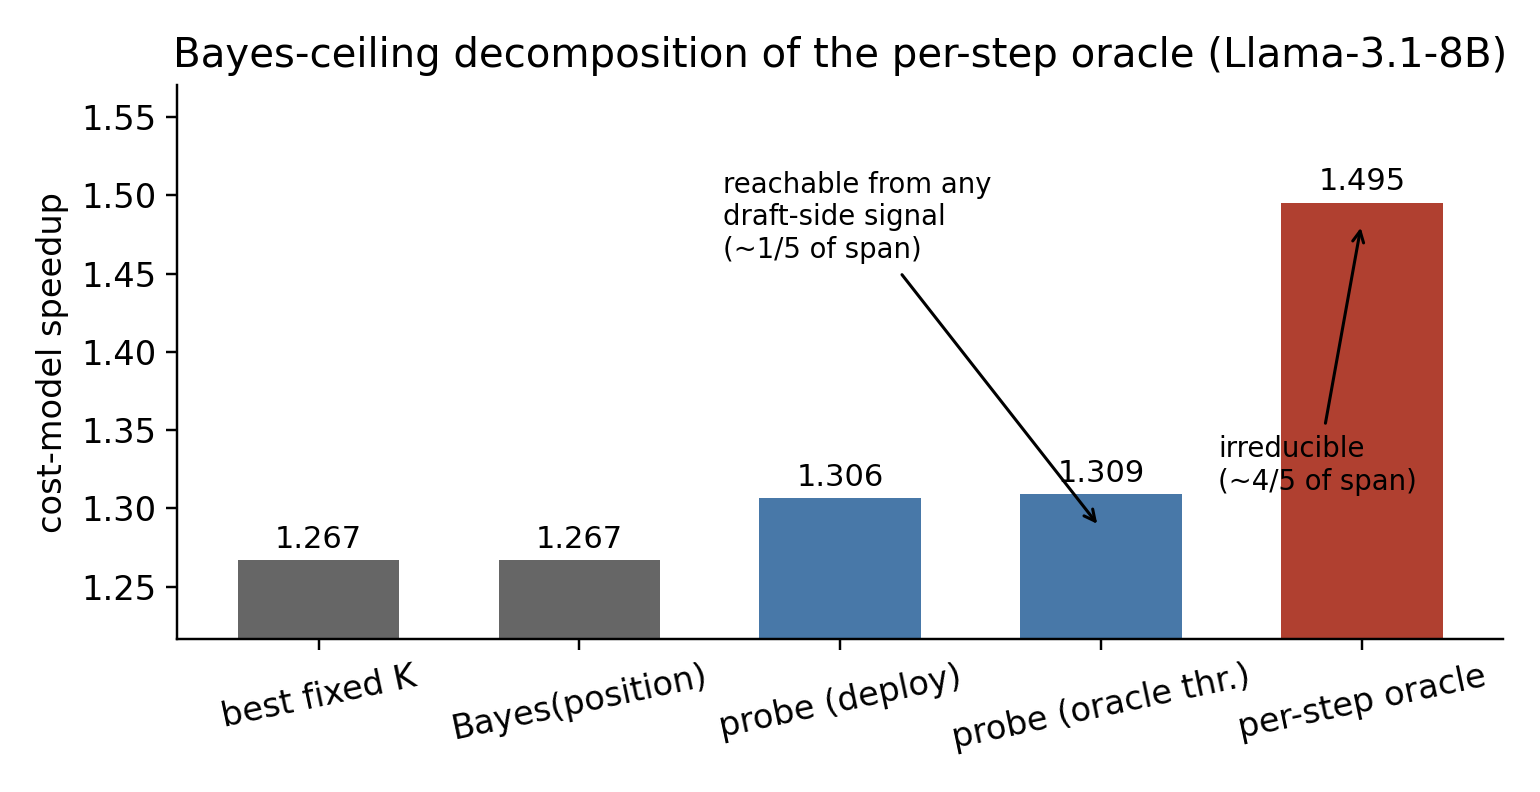
\includegraphics[width=\columnwidth]{figures/fig_decomposition.png}
\caption{The five rungs for Llama-3.1-8B. Only about a fifth of the oracle span is reachable
from any draft-side signal, and Bayes(position) lands exactly on the tuned fixed $K$, which is
the correctness check the ladder has built into it.}
\label{fig:decomp}
\end{figure}

Table~\ref{tab:decomp} and Fig.~\ref{fig:decomp} give three readings.

Bayes(position) is zero everywhere. A static signal cannot beat a tuned fixed $K$, and the
fact that this rung collapses exactly validates the pipeline. It also explains a puzzle in the
literature: position and entropy carry AUC around $0.5$ to $0.58$, which bought earlier methods
nothing because there was nothing there to buy.

The probe with an oracle threshold sits close to the deployable probe and far below the
oracle. Even handed a perfect threshold, a hidden-state probe recovers only about a fifth of
the span. Perfect threshold choice would add between $0.9$ and $3.1\%$ of the span, and we
should be careful with that number, since the deployable and oracle-threshold intervals
overlap in every setting. Treat it as a direction, not a settled result. The other four
fifths is verification-outcome variance that no draft-side signal can see. The oracle
overstates what is achievable by roughly five times.

The reachable part is real for the instruction models, worth $+2.0$ to $3.1\%$ net over a
tuned fixed $K$, and absent for the reasoning head.

\subsection{Controls}
Four checks back the decomposition. \emph{Permutation:} shuffling accept labels across draft
blocks, preserving marginals and prefix structure, collapses Llama recovery from
$+16.8\pm2.7\%$ to $-5.6\pm1.4\%$, a 22.4pp drop. Both arms use the same paired-within-fold
estimator, so they differ only in whether labels belong to their hidden states. That is
signal, not leakage. \emph{Independent re-derivation:} fresh code with different folds, PCA
dimension, seed and policy reproduces the oracle, fixed and ceiling rungs to under 0.1pp and
reproduces the sign of every recovery. Magnitude is implementation-sensitive.
\emph{Measured-cost grounding:} re-scoring at the fitted $C{=}0.072$ leaves Llama at $+17.3\%$
recovery and $+2.9\%$ net. \emph{Detection:} probe AUC runs $0.79$ to $0.88$, against $0.484$
for an earlier 16-dimensional random projection. The weak probe was the earlier limitation,
not the hidden state.

\subsection{A confound we could not remove}
On identical competition-math inputs, Llama-3.1-8B keeps its signal at $+9.5\pm3.7\%$ recovery
and $+2.5\pm1.0\%$ net, while DeepSeek-R1 shows none. That looks like a boundary between model
classes, and we cannot claim it is. The DeepSeek head is simply weaker: accept-length 1.47
against 2.40 on the same task, position-0 acceptance 0.28 against 0.55. A weaker head yields a
smaller ceiling and less detectable signal whatever the model is doing. We therefore scope the
claim to this head. Separating ``reasoning model'' from ``weak draft head'' needs a strong
reasoning-model EAGLE head, and none exists today.

\section{Gate 2: Where the Signal Lives}
\label{sec:gate2}
Gate 1 leaves about a fifth of the span on the table. Gate 2 asks what can reach it, and the
answer narrows quickly.

Cheap logit features are the natural first guess, and they are where most published methods
look. Entropy, margin and SVIP-style statistics recover between $+0.3$ and $8\%$ of the span.
Token position recovers exactly nothing, as Gate 1's correctness check already implied. The
drafter's hidden state is different. A PCA-50 and logistic probe over the full state recovers
$+16.8\pm2.7\%$ and $+17.2\pm2.4\%$ of the oracle for the two instruction models, detecting
rejection at AUC $0.79$ to $0.88$.

The probe family is not the limitation, and we checked it instead of assuming it. On the
same captured traces we compared four probes. These were the 16-dimensional random projection
with gradient boosting we started from, logistic regression on the full hidden state, a
two-layer MLP (256 then 64 units) on the full hidden state, and PCA-50 with logistic
regression. The
random projection detects almost nothing, at AUC $0.484$. The other three land between AUC
$0.79$ and $0.87$, and the MLP does not beat PCA-50 with logistic regression, which is the
probe we report throughout. Capacity was not the missing ingredient.

The scope of this result warrants care. It is a negative result with a precise
address. We looked in the most informative place available on the draft side, using a probe
strong enough to find the signal that weaker probes had missed, and the ceiling barely moved.
Gate 2 therefore closes the search rather than opening a direction: if the hidden state
yields only a fifth of the span offline, no cheaper signal will do better.

\section{Gate 3: Does It Survive Execution?}
\label{sec:gate3}
Offline arithmetic says a few percent is available. We now put it on a clock. vLLM 0.23 has no
per-step draft-length hook, so these tests run in the SafeAILab/EAGLE-3 reference
implementation, in eager PyTorch, with no CUDA-graph penalty. Fixed and adaptive arms share
the same instrumented codepath, which equalises per-step overhead. Llama-3.1-8B, H100, greedy,
otherwise as \S\ref{sec:setup}.

\subsection{A controller on the step's seed state}
A PCA and ridge probe on the step's seed hidden state sets the draft depth. Our first capture
here was incorrect, and the nature of the error is worth recording: seeds were mispaired with
accept-lengths across prompts, because one dangling unverified seed per prompt shifted the
global index. A code audit caught it, the mismatch equalling the prompt count exactly confirmed it, and
we corrected the pairing and reran. With correct pairing the seed carries modest signal,
correlation 0.26. The controller still loses, by $5.7\%$, $2.4\%$ and $5.5\%$ against the best
fixed depth on HumanEval, GSM8K and MT-Bench.

\subsection{Stopping inside the draft loop}
The faithful test is to break the depth loop the moment a per-level probe predicts rejection.
We built a verified copy of the EAGLE-3 draft routine that does exactly this, capping the
shorter tree safely, and confirmed it reproduces coherent generation. The level probe carries
real signal, AUC 0.796, close to the 0.84 we measured offline. Early stopping still loses $5$
to $6\%$ (Table~\ref{tab:inloop}).

\begin{table}[t]
\caption{In-loop probe against fixed full depth (tok/s).}
\label{tab:inloop}
\centering
\small
\begin{tabular}{lrrr}
\toprule
Workload & Fixed (full depth) & In-loop adaptive & Gain \\
\midrule
HumanEval & 144.5 & 137.2 & $-5.1\%$ \\
GSM8K & 128.4 & 121.8 & $-5.1\%$ \\
MT-Bench & 133.4 & 125.3 & $-6.1\%$ \\
\bottomrule
\end{tabular}
\end{table}

The cause is economic rather than statistical. The draft head is cheap, and it produces
tokens faster than the target can verify them, which is consistent with SpecDecode-Bench's 42
to 95\% verification share. That sets the shape of the trade. The speedup on a step is however
deep the drafter gets before the target stops agreeing with it, and stopping early truncates
exactly that. The drafting already done still has to be paid for, but it now buys fewer
accepted tokens, so it stops being an investment and becomes overhead on top of the verify
pass. Optimising away draft compute is the wrong move when drafting is the cheap half. The
offline chain analysis said $+2$ to $3\%$; deployed into the tree engine it inverts sign. That
is failure mode 1 in Table~\ref{tab:failuremodes}, and the literature's evaluation protocol
permits it.

\subsection{Four published-style policies}
\label{sec:zoo}
We extended the test to four stopping policies through the same verified codepath: SVIP-style
entropy, margin, SADDLE/PACER-style cumulative path probability, and a SpecDec++-style trained
hidden probe.

These are reimplementations of each stop \emph{mechanism} rather than ports of the published
systems, and the distinction matters for what the results can be read to mean. Running four
released codebases against each other would confound the stop rule with every other difference
between them: tree construction, draft-head training, engine, tokenizer handling. We instead
hold all of that fixed and change one line, so the arms differ only in what triggers the stop.
That buys comparability at the cost of fidelity. A published system may well outperform our
version of its rule, and a loss in Table~\ref{tab:zoo} is evidence about the mechanism, not
about anyone's implementation of it.

Table~\ref{tab:zoo} gives the verdict, and in the same numbers shows why the
protocol of \S\ref{sec:protocol} was necessary. Read in-distribution, three arms look like
wins. Read on held-out prompts, every one of them loses.

\begin{table}[t]
\caption{The policy zoo (EAGLE-3 tree, Llama-3.1-8B, $B{=}1$), as \% against the strongest
fixed depth in the same run, mean over 3 repeats. Per-cell SE runs $0.2$ to $1.4$\,pp, so
every sign here is larger than its own error bar. The two halves are the same policies, the
same hardware and the same code. They differ only in whether the stop threshold was chosen on
the benched prompts. Under in-distribution selection the best fixed depth is flattered too,
$K{=}8/6/5$ against $K{=}5/5/5$ held-out. These are unpaired 3-repeat runs; for the survivor,
the drift-controlled numbers in Table~\ref{tab:paired} supersede them.}
\label{tab:zoo}
\centering
\small
\setlength{\tabcolsep}{3pt}
\begin{tabular}{lrrrr}
\toprule
Policy & HEval & GSM8K & MT-B & mean \\
\midrule
\multicolumn{5}{l}{\emph{Held-out threshold selection (our protocol)}} \\
\quad Entropy (SVIP-style) & $-2.0$ & $-4.3$ & $-7.7$ & $-4.7$ \\
\quad Saturation tail-pruning & $+0.1$ & $-2.5$ & $-3.2$ & $-1.9$ \\
\quad Hidden probe (SpecDec++) & $-14.0$ & $-14.7$ & $-22.3$ & $\mathbf{-17.0}$ \\
\addlinespace
\multicolumn{5}{l}{\emph{In-distribution selection (the common protocol)}} \\
\quad Entropy (SVIP-style) & $+0.9$ & $+2.6$ & $+1.1$ & $+1.5$ \\
\quad Saturation tail-pruning & $+4.5$ & $+7.3$ & $+7.3$ & $+6.4$ \\
\quad Hidden probe (SpecDec++) & $-15.1$ & $-12.8$ & $-16.2$ & $-14.7$ \\
\bottomrule
\end{tabular}
\end{table}

\begin{figure}[t]
\centering
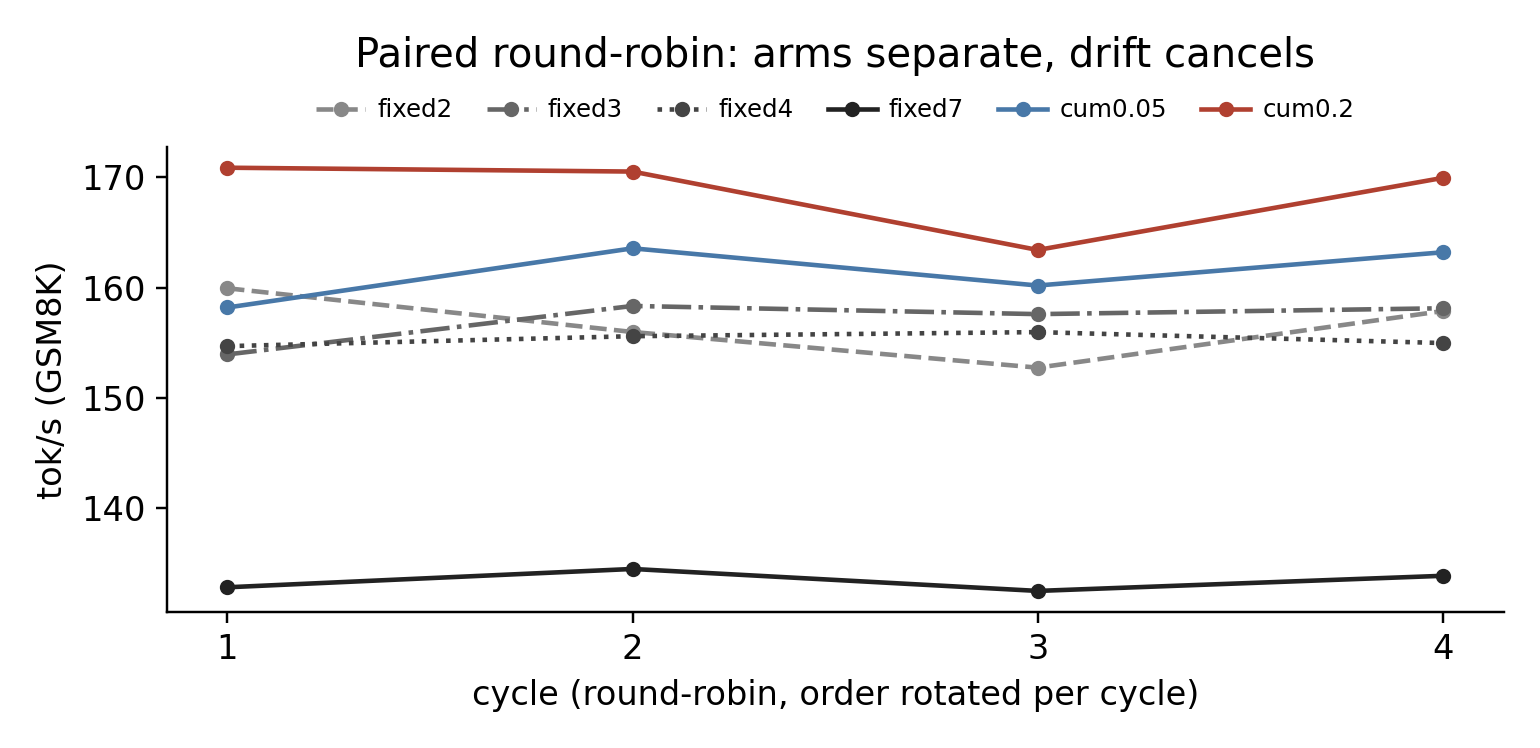
\includegraphics[width=\columnwidth]{figures/fig_paired_protocol.png}
\caption{Why pairing is necessary. Per-cycle raw throughput shows the arms separating and the
container drifting at the same time; paired per-cycle differences cancel the drift that
produced three contradictory sequential answers.}
\label{fig:protocol}
\end{figure}

That is the gate-3 verdict. Every learned or entropy-based per-step policy we tested loses to
a tuned fixed depth, across a range from $2$ to $17\%$. The signal Gate 2 located is real and
acting on it makes things worse.

\section{What Is Left Standing}
\label{sec:survivor}
One arm in Table~\ref{tab:zoo} behaves differently from the rest, and it is the one that uses
no learned signal at all. Saturation tail-pruning stops drafting when the cumulative best-path
probability the drafter has already computed falls below a threshold. Zero model cost, no
training, and the policy family already exists in prior art \cite{saddle,pacer,ddd}. Under the
paired protocol it wins (Table~\ref{tab:paired}).

\begin{table}[t]
\caption{Paired verdict on held-out prompts against the strongest per-workload fixed depth.
Saturation tail-pruning, threshold 0.05 selected on train.}
\label{tab:paired}
\centering
\small
\begin{tabular}{lrr}
\toprule
Workload & Paired gain & Cycles positive \\
\midrule
GSM8K & $+3.58\% \pm 0.32$ & 4/4 \\
MT-Bench & $+4.77\% \pm 0.50$ & 4/4 \\
HumanEval & $+2.90\% \pm 1.83$ & 3/4 \\
\bottomrule
\end{tabular}
\end{table}

It wins at a realized mean depth of 5.62 against a fixed 7 to 8. Outputs are identical, the
verified tree size is unchanged, and the fixed arms run the same instrumented codepath, so the
gain is pure draft-iteration savings.

The decomposition explains why this one works when prediction does not, and the explanation
comes down to what it costs to ask. Predicting acceptance requires anticipating realization
variance, which \S\ref{sec:gate1} showed is mostly irreducible, and the probe has to run PCA
and a logistic model over the hidden state at every level to attempt it. Saturation pruning
multiplies the current token probability into the running product for its branch, a quantity
the tree search has already computed. Its decision is free.

That difference is measurable, not rhetorical. In the held-out zoo run the probe drafts
to a realized depth of $6.95$, which lets us compare it against a fixed depth of 7 doing the
same drafting and the same verification. The probe is $10$ to $13\%$ slower on the three
workloads ($120.9$ against $138.4$ tok/s on HumanEval, $115.6$ against $129.2$ on GSM8K, $85.0$
against $96.0$ on MT-Bench). That gap is the cost of asking the question. Set against a
reachable gain that Gate 1 caps at a few percent, the decision costs several times what the
decision is worth. Saturation pruning wins the same comparison by not paying it.

\subsection{How far the result travels}
\emph{Cross-head.} On the weaker DeepSeek-R1-Distill head, accept-length about 1.5 against
Llama's 2.4, the same protocol yields a tie: $-0.7\%$, $-0.9\%$ and $+1.4\%$, none
significant, at realized depth 6.19. It prunes about 0.8 levels where Llama prunes 1.4.
Tail-pruning pays when a strong head makes deep fixed budgets frequently wasteful, and on a
weak head there is less tail to prune. This run also surfaced failure mode 4: one cycle was
contaminated by an intra-cycle throughput step-change, with the fixed arms jumping 14 to 18\%
mid-cycle, which pairing does not cancel. Robust use of the protocol wants six or more cycles,
or median-of-cycles statistics.

\emph{Production engine.} Since vLLM exposes no per-step hook, we patched the live draft loop
of its V1 engine, locating it by stack-tracing from a hooked draft-head call. This was necessary because vLLM 0.23 ships a parallel legacy spec-decode package that is dead code in
this configuration. Patching it produces a plausible, silent no-op that only an arm-separation
check catches, and our first attempt was invalidated exactly this way and quarantined. All
arms share the patched codepath and pay verification for all 7 slots, which isolates
draft-side savings under equal verify cost. The gates hold: 19\% separation between fixed
arms, and the strongest fixed arm lands at $k{=}2$ to $3$, matching the independently tuned
production $K{=}2$. Against the strongest fixed arm, cum(0.2) gains $+6.4\%$, $+7.5\%$ and
$+2.9\%$ on Llama-3.1-8B at adaptive mean draft 2.3. On Qwen3-14B it is a tie to slight win,
$+1.3\%$, $+0.3\%$ and $+0.7\%$ at mean draft 3.05, and the aggressive threshold hurts there.

\emph{Fair baselines.} Padding the fixed arms to 7 slots could in principle hand the adaptive
arm a verification advantage it has not earned, which is failure mode 6. So we loaded three
engines in one process, native $K{=}2$ and $K{=}3$ each with its true verification budget plus
the patched $K{=}7$ cum engine, and round-robined across engines on three fresh containers
under vLLM v0.24. Each native engine provably drafts exactly its $K$, and realized draft
lengths are bit-identical across containers, since greedy decoding is deterministic and only
the clock varies. The result is positive or tied in 9 of 9 workload cells
(Table~\ref{tab:fairbase}). Cross-container spread exceeds the within-run error bars, with
MT-Bench alone spanning $-0.2$ to $+3.5$ across three identically configured containers. That
is the strongest argument in this paper against trusting any single-container benchmark
number, including ours.

\begin{table}[t]
\caption{Fair-baseline replication: paired gain of cum(0.2) over the strongest native engine,
each drafting its true $K$, on three fresh containers. Positive or tied in 9/9 cells, and the
worst is a tie.}
\label{tab:fairbase}
\centering
\small
\setlength{\tabcolsep}{4pt}
\begin{tabular}{lrrrr}
\toprule
Workload & cont.\ 1 & cont.\ 2 & cont.\ 3 & mean$\pm$SE \\
\midrule
HumanEval & $+6.9$ & $+6.6$ & $+3.3$ & $+5.6{\pm}2.0$ \\
GSM8K & $+7.1$ & $+8.4$ & $+1.8$ & $+5.7{\pm}2.9$ \\
MT-Bench & $+3.5$ & $-0.2$ & $+2.7$ & $+2.0{\pm}1.6$ \\
\bottomrule
\end{tabular}
\end{table}

The padded and native baselines agree because verification is flat in $K$, and we measured
that rather than assuming it. A verify microbench under HF-eager isolation shows one
kernel-regime step, from the non-speculative single-token forward at $q{=}1$, 15.8\,ms, to the
multi-token path. After that it is flat: $q{=}2$ to $q{=}8$ runs 18.5 down to 18.2\,ms at
$B{=}1$.
Native $K{=}2$'s $q{=}3$ and the padded arm's $q{=}8$ differ by under 1\%. The honest headline
is therefore $+2$ to $5\%$ with one of three workloads a wash, MT-Bench at $+2.0\pm1.6$ and a
worst cell of $-0.2\pm2.0$, and never a significant loss.

\emph{Temperature and batch.} At $T{=}0.8$ with seeded sampling and rejection-sampling
verification the win survives, $+5.4\%$, $+2.1\%$ and $+1.5\%$, all positive-significant, at
realized depth 2.24. Sampling lowers acceptance, so saturation fires earlier, which is the
direction the mechanism predicts. With batch the gain decays monotonically
(Fig.~\ref{fig:batch}): $+2$ to $6\%$ at $B{=}1$, about $+1\%$ at $B{=}4$, and 0 to $-3\%$ at
$B{=}8$, with realized depth drifting up from 2.3 to 2.68. We use a batch-level
mean-confidence rule because per-request ragged stopping is impossible in a batch-synchronized
draft loop, which is itself a finding about adaptive-length methods in serving engines. The
microbench identifies the mechanism: verify latency stays flat even at $B{=}8\times q{=}8$, so
the decay is not verification-cost growth. It is the batch-synchronized mean stop wasting
per-request adaptivity, forcing rejects on requests whose chains were still alive, and the
rising realized depth is that compromise made visible.

\begin{figure}[t]
\centering
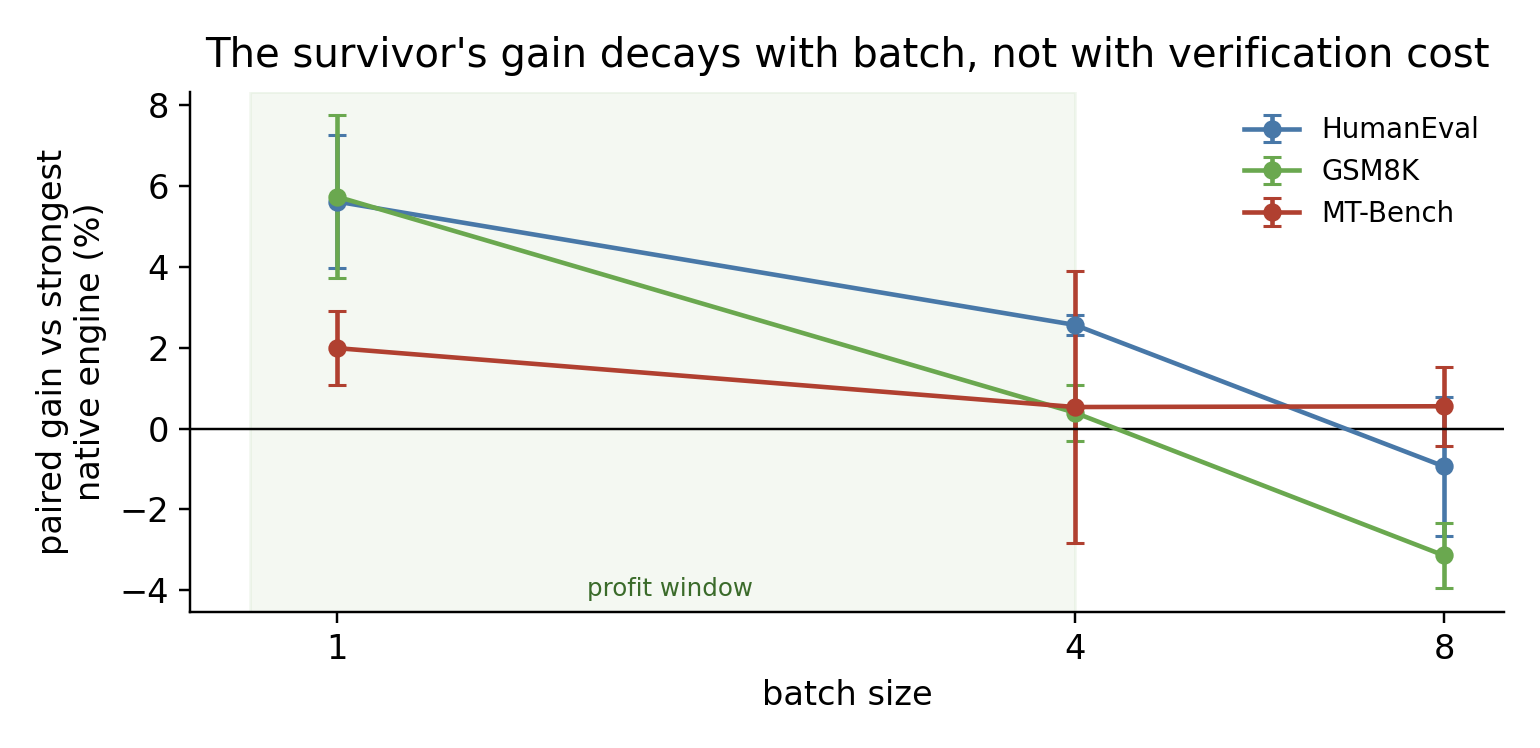
\includegraphics[width=\columnwidth]{figures/fig_batch_decay.png}
\caption{The survivor's profit window. Paired gain over the strongest native engine decays
from $+2$ to $6\%$ at $B{=}1$ to between 0 and $-3\%$ at $B{=}8$. The verify microbench rules
out verification-cost growth as the cause; the batch-synchronized mean stop is what erodes it.}
\label{fig:batch}
\end{figure}

The practitioner's question is whether this can be switched on in production, and for a
batched deployment our answer is no, with one qualification.

The qualification is that we tested the batch-synchronized version, not a ragged engine that
stops each request independently. Such an engine is buildable and might decay differently. We
did not build one, so the deployable number is open rather than settled. What we can claim is
that the profit window we observed is latency-sensitive low-batch serving, $B \lesssim 4$,
consistent with our own batch-collapse result (\S\ref{sec:supporting}) and with
SpecDecode-Bench's batch-dependent optimal draft lengths \cite{specdecodebench}. Both
directions were stated in advance of the runs as consequences of the saturation mechanism.

None of this contradicts the methods that do pay off in production. Nightjar \cite{nightjar}
and TurboSpec \cite{turbospec} adapt at the load level, deciding whether to speculate at all
given batch size and system load, which is a different lever from per-step draft length. Our
batch-collapse data supports that choice: by $B{\geq}32$ the best-$K$ gap is exactly zero, so
there is nothing left for a per-step controller to win, while the decision of whether to
speculate still has room in it.

Pulling the settings together (Fig.~\ref{fig:survivor}): a free, signal-less saturation-pruning
policy at a conservative threshold ties or beats the tuned fixed baseline everywhere we
tested. Llama chain $+2.9$ to $7.5\%$, Llama tree $+2$ to $5\%$, Qwen3 chain $+0.3$ to
$1.3\%$, weak head about zero. Every learned acceptance-prediction policy loses everywhere.

\begin{figure}[t]
\centering
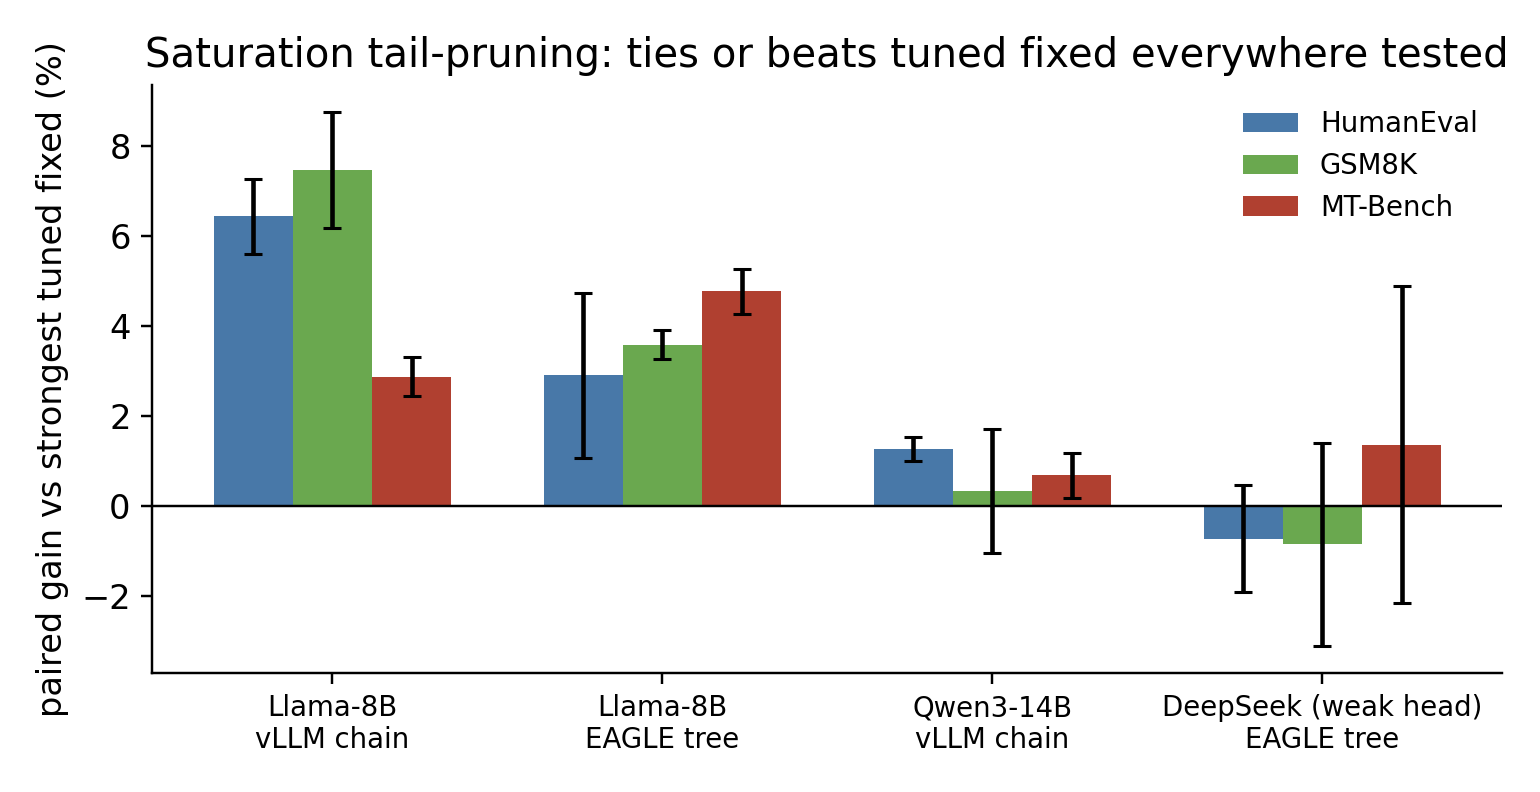
\includegraphics[width=\columnwidth]{figures/fig_survivor.png}
\caption{The survivor across settings. Saturation tail-pruning ties or beats the strongest
tuned fixed baseline everywhere tested, and the gain scales with draft-head strength.}
\label{fig:survivor}
\end{figure}

Adaptive \emph{deepening} beyond the default budget is a different lever and we did not test
it (cf.\ TALON \cite{talon}).

\section{Supporting Results}
\label{sec:supporting}
\emph{Batch collapse.} Adaptive headroom shrinks as batch grows. At $B{=}16$ the best-$K$ gap
over $K{=}1$ is still $+5$ to $11\%$; at $B{\geq}32$ it is exactly zero on every workload. The
serving regime removes even the theoretical motivation for per-step control. This also bounds
the gate-3 result, since verification dominance grows with batch, so tail-pruning's draft-side
savings can only shrink. The $+2$ to $5\%$ is a $B{=}1$ ceiling.

\emph{Long context.} Headroom at 8K is gated by draft quality, not KV bandwidth. Qwen3-14B
holds $1.31$ to $1.39\times$ at ctx$=$8192, and even at $B{=}32$ keeps a $+3\%$ gap, the one
cell consistent with MagicDec \cite{magicdec}. Llama-8B and DeepSeek collapse to about
$1.0\times$ as their heads' acceptance falls to roughly 1.1 tokens per step.

\emph{Reconciling prior gains.} AdaEAGLE, SVIP, SpecDec++ and DDD report 2 to 8\% against
default-$K$ or $K{=}1$ baselines. Against our tuned fixed $K$ the per-request oracle, which
is the relevant bound for a method that effectively selects one depth per request, is only
$+2.0\%$, and every online controller we ran went negative (Table~\ref{tab:bandit}).

\begin{table}[t]
\caption{Online \emph{per-request} controllers against a tuned fixed depth: each policy picks
one $K$ per prompt and adapts across prompts, which is a different lever from the per-step
stopping policies of \S\ref{sec:gate3}. Run in a separate harness and worth distinguishing
from the rest of the wall-clock work: vLLM 0.23 in the chain regime with
\texttt{num\_speculative\_tokens}=7, rather than the SafeAILab eager tree implementation, and
over 90 prompts (30 per workload across HumanEval, GSM8K and MT-Bench) rather than the 10
held-out prompts the \S\ref{sec:gate3} tables use. Llama-3.1-8B with EAGLE-3, H100, $B{=}1$,
greedy, measured wall-clock. Every reactive controller loses, and the per-request oracle
bounds what any of them could have won at $+2.0\%$.}
\label{tab:bandit}
\centering
\small
\begin{tabular}{lrr}
\toprule
Policy & net speedup & vs best fixed \\
\midrule
Fixed $K{=}2$ (tuned baseline) & $1.538\times$ & --- \\
UCB (BanditSpec-style) & $1.463\times$ & $-4.9\%$ \\
$\epsilon$-greedy & $1.432\times$ & $-6.9\%$ \\
Acceptance-history & $1.394\times$ & $-9.3\%$ \\
\midrule
Oracle (per-request) & $1.569\times$ & $+2.0\%$ \\
\bottomrule
\end{tabular}
\end{table}

We report these in some detail because the failure has a cause worth sharing, and because our
implementations are simple enough that someone with a better one may well do otherwise. Two
measurements from the same traces explain the pattern. First, the prize is capped: the
per-request oracle is $+2.0\%$, so a controller has to find the right depth almost immediately
or its exploration is unrecoverable. Reactive bandits explore by construction, and here there
is nothing to amortise that exploration against. Second, the quantity they are trying to learn
barely persists. Across 1{,}295 decode steps the accept-run distribution is heavily
zero-inflated, with $61\%$ of steps accepting no draft token at all, and the lag-1
autocorrelation of the accept-run is only $0.247$. What the last step taught is a weak
guide to the next one, so an online learner spends its budget tracking something close to
noise.

That is the learning we would most like others to test. A stronger bandit, a better-designed
exploration schedule, or a setting with higher autocorrelation might change this. We would be
glad to see it, and the traces are released so that a counter-example can be produced against
the same data rather than a new capture.

We read this as a baseline effect, not an error in those papers. Their measurements are
correct for the baselines they used, and moving off a poorly chosen fixed depth is a real
improvement worth reporting. The difficulty is that tuning the fixed depth captures much of
the same improvement, so the two do not add: a practitioner who tunes $K$ first should not
expect the published increment on top. What our decomposition adds is an account of why the
remainder is so thin once tuning is done, and that account applies to our own probe as much as
to anyone else's method.

\section{Discussion}
Our advice to anyone setting out to shorten drafts from a learned signal is to compute the
ceiling before building the predictor. The gap between a tuned fixed depth and the per-step
oracle is the number that motivates the field, and it is the wrong number to aim at. Split it
first into the part a draft-side signal could reach and the part that is verification-outcome
variance no draft-side signal can see. On every model pair we measured, the second part is
about four fifths of the total, and what remains is small enough that a predictor has to be
nearly free to be worth running. That split costs one capture run and an afternoon of
analysis. It is much cheaper than the months we spent finding out the other way, and on our
pairs it would have said no.

Two things this advice does not cover. It concerns the shortening lever only: adaptive
deepening beyond the default budget is untested here (cf.\ TALON \cite{talon}). And it
concerns draft-side signals only, since a quantity available after verification is a different
question, if not a usable one for this purpose.

The oracle plots themselves are real. They are simply a measure of hindsight, and the reachable
slice inside them is genuinely present in the hidden state, worth a few percent offline and
negative end-to-end once a learned policy has to pay for itself. The one adaptive lever that
pays needs no signal at all.

That pattern explains something about where the field went in 2025 and 2026. Work moved toward
load-level adaptation, deciding whether to speculate based on batch and system load, and our
batch-collapse data confirms that is the profitable lever. Signal-level length controllers keep
failing against tuned baselines for a structural reason, not because nobody has found the
right feature yet.

For practitioners, the advice is short. Ship a tuned, deep fixed draft length plus free
saturation tail-pruning, and spend the adaptivity budget at the serving level instead of on
per-step prediction. For anyone evaluating such methods, at the $\pm5\%$ scale these claims
occupy, mechanism-matched simulators, held-out threshold selection and paired drift-controlled
timing are not optional extras.

\section{Limitations}
\begin{itemize}
\item Offline gains are cost-model figures at $B{=}1$: net $+2.0$ to $3.1\%$, recovery
$+16.8\pm2.7\%$ and $+17.2\pm2.4\%$ for the two instruct models under the corrected paired
estimator. End-to-end, learned early-stopping does not realize them.
\item The probe is trained in-distribution, on held-out generations from the same models and
workloads. Cross-workload and cross-model transfer is untested.
\item The reasoning-head null is confounded by lower base acceptance (\S\ref{sec:gate1}) and is
scoped to that head.
\item ``Irreducible'' means irreducible from draft-side signals. Privileged post-verification
quantities are a different question.
\item Gate 3 tests early stopping only. Adaptive deepening beyond the default budget is
untested. Single-pass timings in \S\ref{sec:gate3}'s first two experiments carry a noise bar
of about 2\%; the policy-zoo verdict uses the paired protocol.
\item The tail-pruning positive holds for a strong instruction head on an H100 at $B{=}1$, with
HumanEval borderline, and ties on the weaker DeepSeek-R1-Distill head. The gain is
head-dependent and scoped accordingly.
\item Wall-clock work uses the eager reference implementation, since vLLM has no per-step hook.
Relative fixed-versus-adaptive comparisons are valid; absolute tok/s is lower than vLLM. This
also bounds the probe-overhead measurement in \S\ref{sec:survivor}: a per-level Python call is
near its worst case in eager mode, and a fused or batched implementation would cost less. The
direction of that result is safe, since the probe must do strictly more work than reading a
number the tree already holds, but the $10$ to $13\%$ magnitude is specific to this engine.
\item The wall-clock samples are small: 10 held-out prompts per workload at 128 max new
tokens, 8 in the batched runs. Precision comes from repetition and pairing rather than from
prompt count, and the reported error bars are over cycles, not over prompts. Cross-container
spread in Table~\ref{tab:fairbase} exceeds the within-run bars, which is the honest statement
of how far these magnitudes should be trusted.
\end{itemize}

\section{Conclusion}
We followed the speedup that adaptive draft length promises and traced where it is lost. Against a
tuned fixed draft length, about $80\%$ of the celebrated per-step oracle is irreducible from
any draft-side signal. The reducible fifth lives in the drafter's hidden state, is worth $+2$
to $3\%$ offline for instruction-model heads, and loses $2$ to $17\%$ end-to-end when a policy
acts on it, because verification dominates execution. We audited four policies in wall-clock under a
paired, drift-controlled protocol, itself forced on us by six evaluation failure modes. It
leaves exactly one survivor: signal-free saturation tail-pruning, worth $+2$ to $5\%$ at zero
model cost, with one of three workloads a wash and only at low batch. The deployable recommendation
is a tuned deep draft plus free tail-pruning. The learned per-step signal the field keeps
chasing is real, we know where it lives, and for the shortening lever it is not worth acting
on.

\section*{Reproducibility}
Everything below is released at \url{https://github.com/pramodjella/speculative-decoding-draft-length-audit},
including the raw per-run JSON behind every table and figure in this paper;
\texttt{DELIVERABLES.md} maps each result (E1--E6) to the script and artifact that produced it.
Hidden-state capture (\texttt{modal\_eagle3\_hidden\_full\_capture.py}); the decomposition
(\texttt{analyze\_bayes\_ceiling\_paired.py}, the paired-within-fold version that carries the
nesting and position self-tests) with its permutation control and independent re-derivation;
cost grounding (\texttt{measured\_cost\_ground.py}); wall-clock harnesses
(\texttt{modal\_eagle\_wallclock.py}, \texttt{modal\_eagle\_inloop.py}); the policy zoo and the
paired protocol (\texttt{modal\_eagle\_zoo\_verify.py}, \texttt{modal\_eagle\_paired.py}); and the
fair-baseline native-engine replication (\texttt{modal\_vllm\_fairbase.py}). A single
\texttt{scripts/check\_stale.sh} gate guards the shipped documents against retired numbers.

\begin{thebibliography}{00}
\bibitem{leviathan2023spec} Y. Leviathan, M. Kalman, and Y. Matias, ``Fast inference from transformers via speculative decoding,'' ICML, 2023.
\bibitem{chen2023spec} C. Chen et al., ``Accelerating large language model decoding with speculative sampling,'' arXiv:2302.01318, 2023.
\bibitem{li2024eagle} Y. Li et al., ``EAGLE: Speculative sampling requires rethinking feature uncertainty,'' ICML, 2024.
\bibitem{li2024eagle2} Y. Li et al., ``EAGLE-2: Faster inference of language models with dynamic draft trees,'' EMNLP, 2024.
\bibitem{li2025eagle3} Y. Li et al., ``EAGLE-3: Scaling up inference acceleration of large language models via training-time test,'' arXiv:2503.01840, 2025.
\bibitem{zhang2024svip} Z. Zhang et al., ``SVIP: Self-verification length policy for speculative decoding,'' arXiv:2411.18462, 2024.
\bibitem{specdec} K. Huang et al., ``SpecDec++: Boosting speculative decoding via adaptive candidate lengths,'' arXiv:2405.19715, 2024.
\bibitem{disco} J. Mamou et al., ``Dynamic speculation lookahead accelerates speculative decoding of large language models,'' arXiv:2405.04304, 2024.
\bibitem{hou2025banditspec} Y. Hou, F. Zhang, C. Du, X. Zhang, J. Pan, T. Pang, C. Du, V. Y. F. Tan, and Z. Yang, ``BanditSpec: Adaptive speculative decoding via bandit algorithms,'' ICML, arXiv:2505.15141, 2025.
\bibitem{adaedl} S. Agrawal, W. Jeon, and M. Lee, ``AdaEDL: Early draft stopping for speculative decoding of large language models via an entropy-based lower bound on token acceptance probability,'' NeurIPS Workshop on Efficient Natural Language and Speech Processing, arXiv:2410.18351, 2024.
\bibitem{dsde} M. Yang, J.-Y. Choi, K. Moon, M. Jang, and E. Jeon, ``DSDE: Dynamic speculative decoding with KLD stability for real-world serving,'' arXiv:2509.01083, 2025.
\bibitem{ddd} O. Brown et al., ``Dynamic depth decoding: Faster speculative decoding for LLMs,'' arXiv:2409.00142, 2024.
\bibitem{saddle} R. Wang, Q. Wang, H. Liu, L. Zheng, X. Liao, H. Jin, and J. Xue, ``Adaptive draft sequence length: Enhancing speculative decoding throughput on PIM-enabled systems,'' HPCA, 2026.
\bibitem{pacer} S. Zhang, Y. Zhang, Z. Zhu, H. Wang, D. Ma, D. Zhang, L. Chen, and K. Yu, ``PACER: Blockwise pre-verification for speculative decoding with adaptive length,'' arXiv:2602.01274, 2026.
\bibitem{talon} T. Liu, Q. Lv, Y. Shen, X. Sun, and X. Sun, ``TALON: Confidence-aware speculative decoding with adaptive token trees,'' arXiv:2601.07353, 2026.
\bibitem{nightjar} R. Li, Z. Zhang, L. Zhang, H. Wang, X. Fu, and Z. Lai, ``Nightjar: Dynamic adaptive speculative decoding for large language models serving,'' arXiv:2512.22420, 2025.
\bibitem{turbospec} X. Liu, J. Park, L. Hu, W. Kwon, Z. Li, C. Zhang, K. Du, X. Mo, K. You, A. Cheung, Z. Deng, I. Stoica, and H. Zhang, ``TurboSpec: Closed-loop speculation control system for optimizing LLM serving goodput,'' arXiv:2406.14066, 2025.
\bibitem{specdecodebench} X. Liu, J. Yu, J. Park, I. Stoica, and A. Cheung, ``Speculative decoding: Performance or illusion?'' arXiv:2601.11580, 2026.
\bibitem{magicdec} J. Chen et al., ``MagicDec: Breaking the latency-throughput tradeoff for long context generation with speculative decoding,'' arXiv:2408.11049, 2024.
\end{thebibliography}

\end{document}
